\chapter{Follow-up and Future work}\label{chap:discuss}

The work presented here has been and continues 
to be extended in a number of different theoretical 
and empirical directions.
Earlier work has already been leveraged in published work,
and more recent chapters
have led to interesting
continuing avenues of research.

\section{Analyzing Disease Trends in Functional MRI via Covariance Trajectories}

Work in Chapters~\ref{chap:covtraj} and \ref{chap:ott} has been further developed for a number of other applications.
Ideas have contributed
to the understanding and modeling of uncertainty
in recurrent models~\citep{spgru},
and more generally towards efficient
Bayesian methods for deep Monte Carlo methods~\citep{mcreparam}.
Applications based on modeling disease progression
as a function of both static and time-varying 
variables was extended to ``deepify-ing" mixed effects models~\citep{deepmem}.
Interesting developments on the tensor decomposition side
have led to work combining ideas
in earlier work inarchitecture search~\citep{submodarch}
with such compression methods,
influencing high visibility publications by peers~\citep{xiong2021mobiledets}.

More directly, the covariance trajectory analysis
methods have been extended 
to the analysis of other Alzheimer's Disease populations~\citep{isbi},
and work on understanding and localizing temporal lobe epilepsy
measured over resting-state functional MRI acquisitions is under review.

\subsection{Brain Network Abnormalities in Alzheimer's Disease}
Rs-fMRI has been shown to be a valuable neuroimaging modality to study the pathophysiological mechanisms and effects of Alzheimer's Disease. 
However, most existing brain network modeling frameworks for rs-fMRI often do not account for the combined statistical and temporal dependencies underlying dynamic functional connectivity (dFC) in a statistically robust manner, 
which may be limiting our understanding of altered brain organization in disease.
To address these issues, in this work we demonstrate that
the covariance trajectory methods above can characterize dFC as covariance trajectories on the Riemannian manifold.

In this follow-up work,
we leverage a different setup of the trajectory analysis in Chapter~\ref{chap:covtraj}. Here,
we have a much larger number of timepoints:
compared to patient site visits,
we have functional MRI measurements
occurring at a rate of approximately once per second for scans ranging from 5 to 10 minutes.
While the methods above can be applied,
the computational cost, while not exponential,
still grows at a rate infeasible 
for this application.

To address this, we construct a ``windowed" approach, where we set specific window sizes and stride lengths such that our trajectory spans the length of the scan,
and smoothly estimates the continuous trajectory through overlapping samples.
We fit the trajectories for each subject and take corresponding means for the likelihood statistics and follow the hypothesis testing as above.
Experimental results demonstrated that the approach is capable of identifying differential effects in large-scale functional networks altered in Alzheimer's Disease in a way that overcomes statistical challenges common with many neuroimaging studies.

\begin{figure}
	\centering
	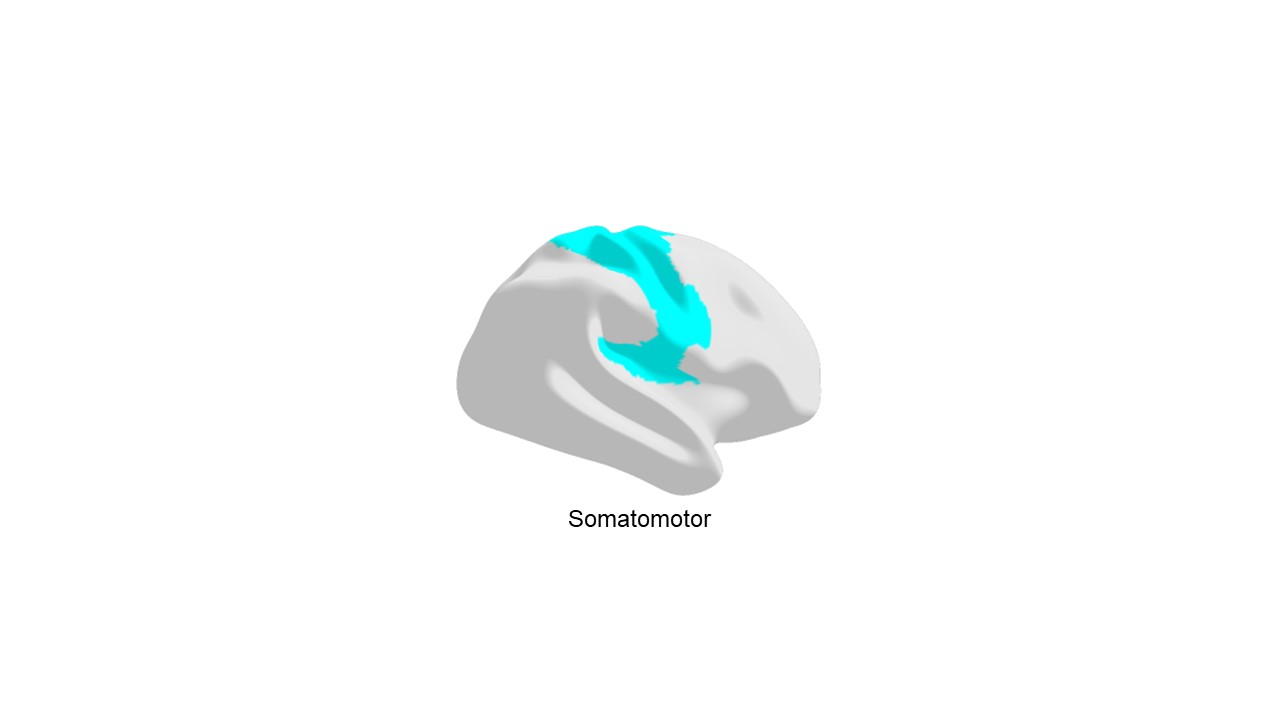
\includegraphics[width=0.3\columnwidth, trim={11cm 5cm 9cm 5cm}, clip]{7_conclude/figs/Results_Network1.jpg}
	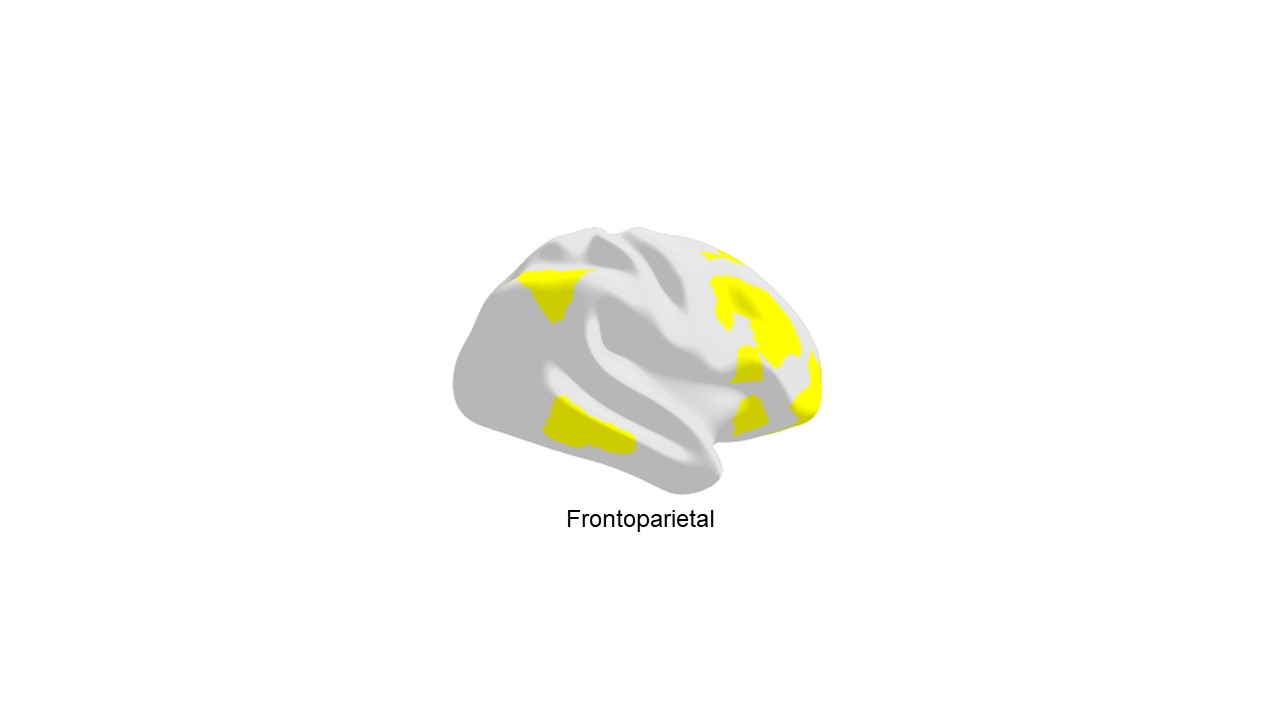
\includegraphics[width=0.3\columnwidth, trim={11cm 5cm 9cm 5cm}, clip]{7_conclude/figs/Results_Network2.jpg}
	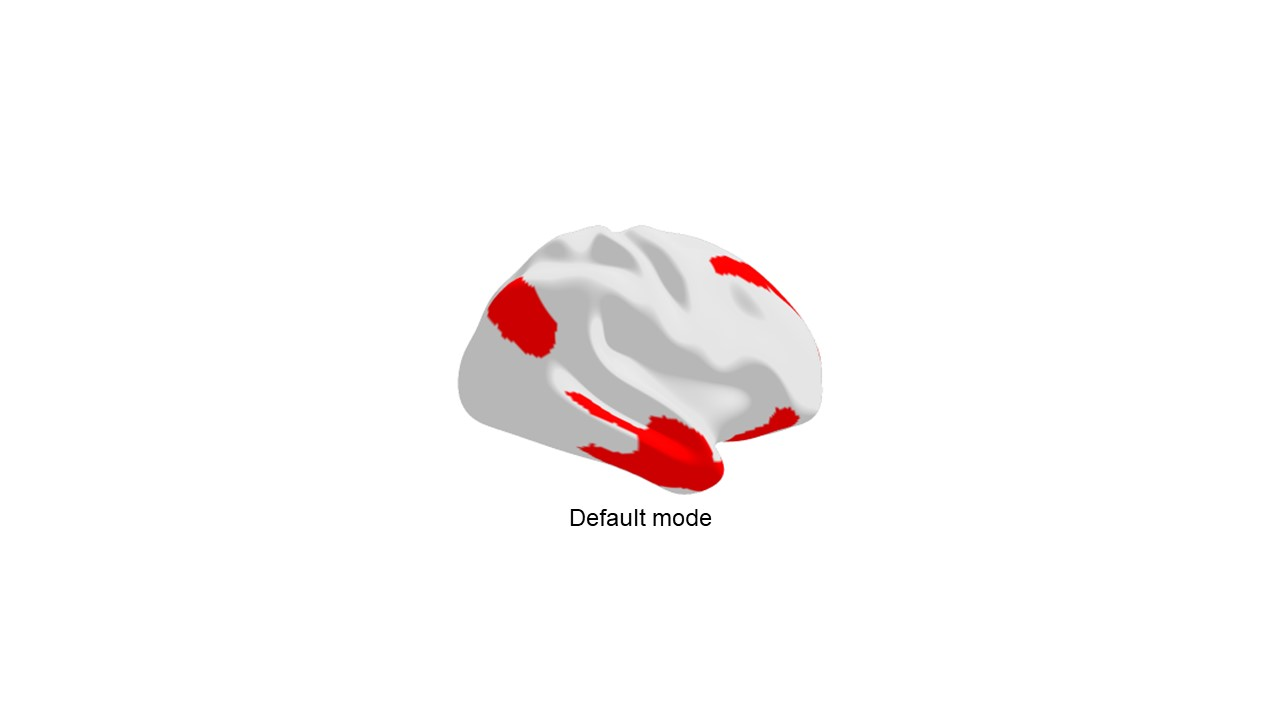
\includegraphics[width=0.3\columnwidth, trim={11cm 5cm 9cm 5cm}, clip]{7_conclude/figs/Results_Network3.jpg}
	
	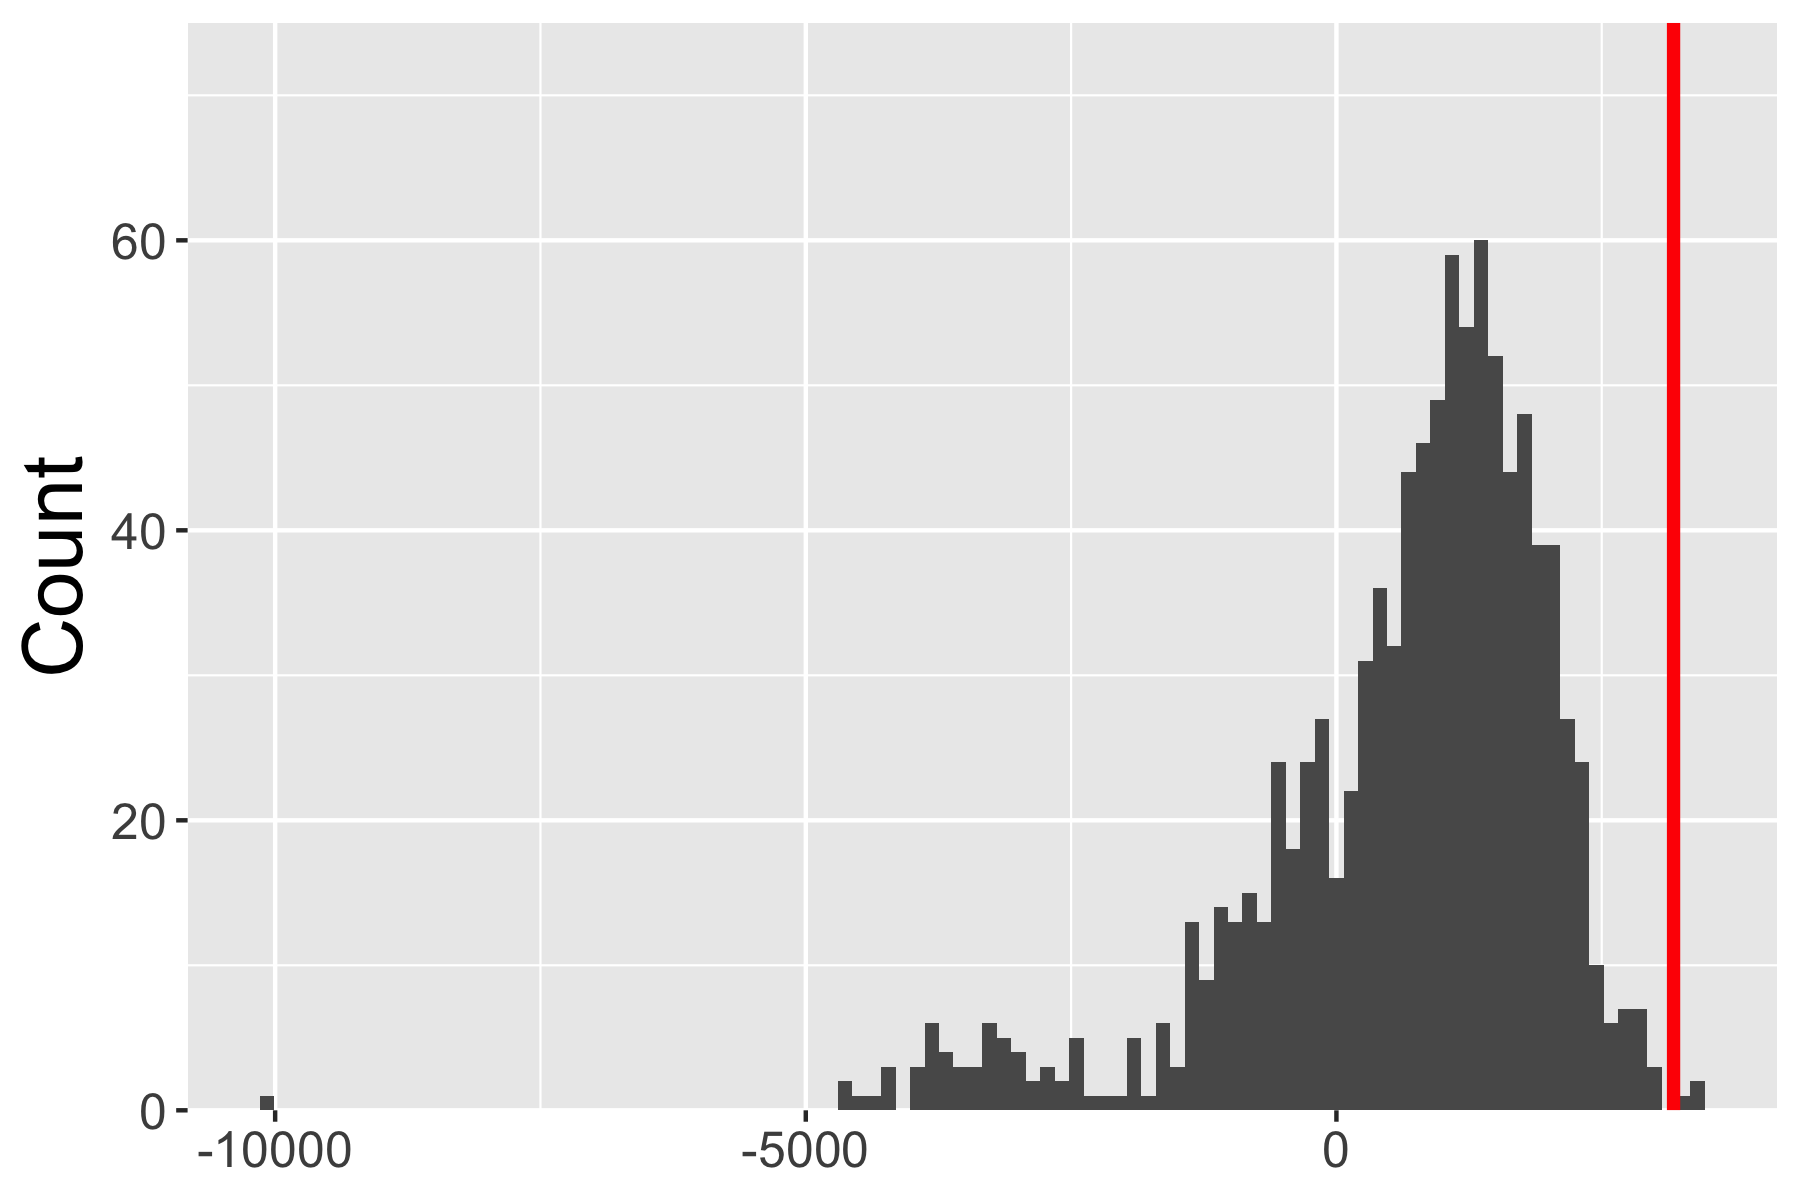
\includegraphics[width=0.3\columnwidth, trim={4cm 1cm 2cm 5cm}, clip]{7_conclude/figs/X1.png}
	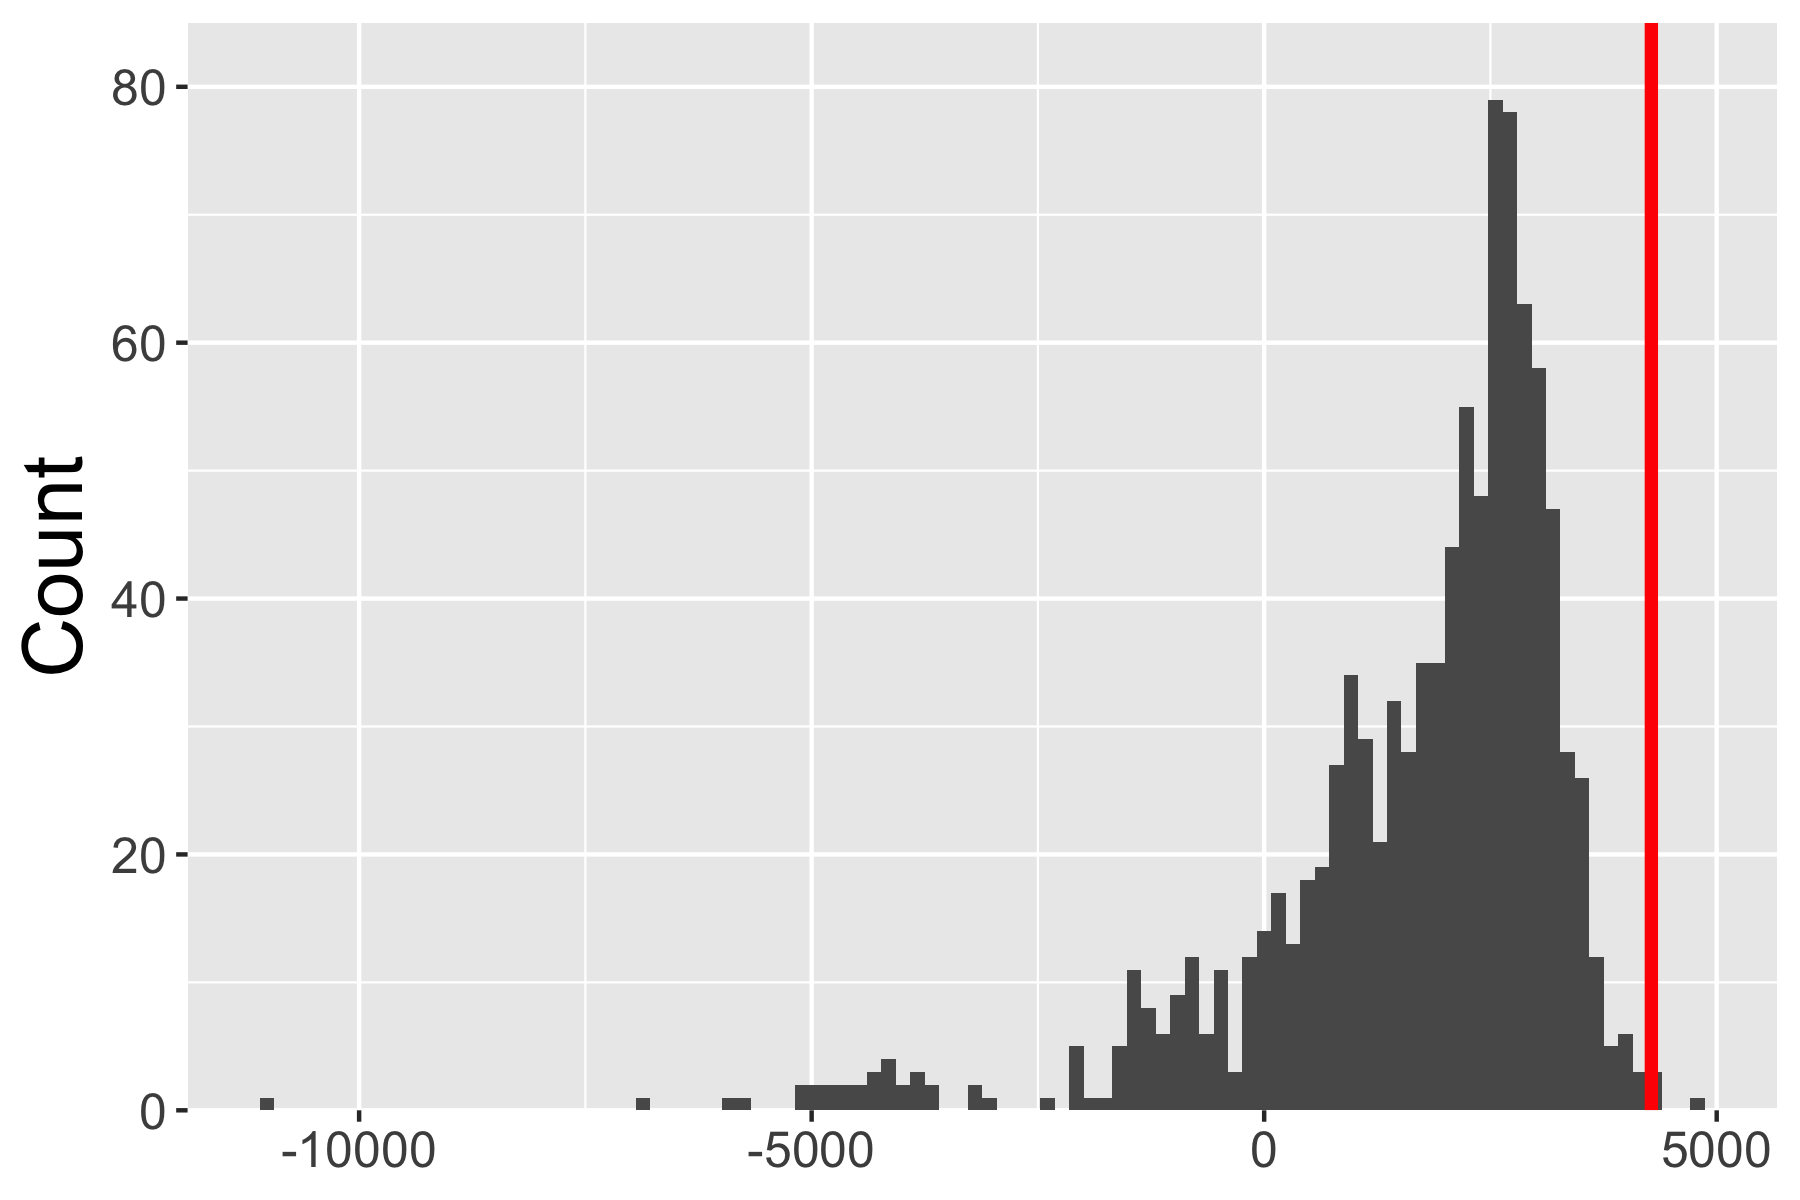
\includegraphics[width=0.3\columnwidth, trim={4cm 1cm 2cm 5cm}, clip]{7_conclude/figs/X2.png}
	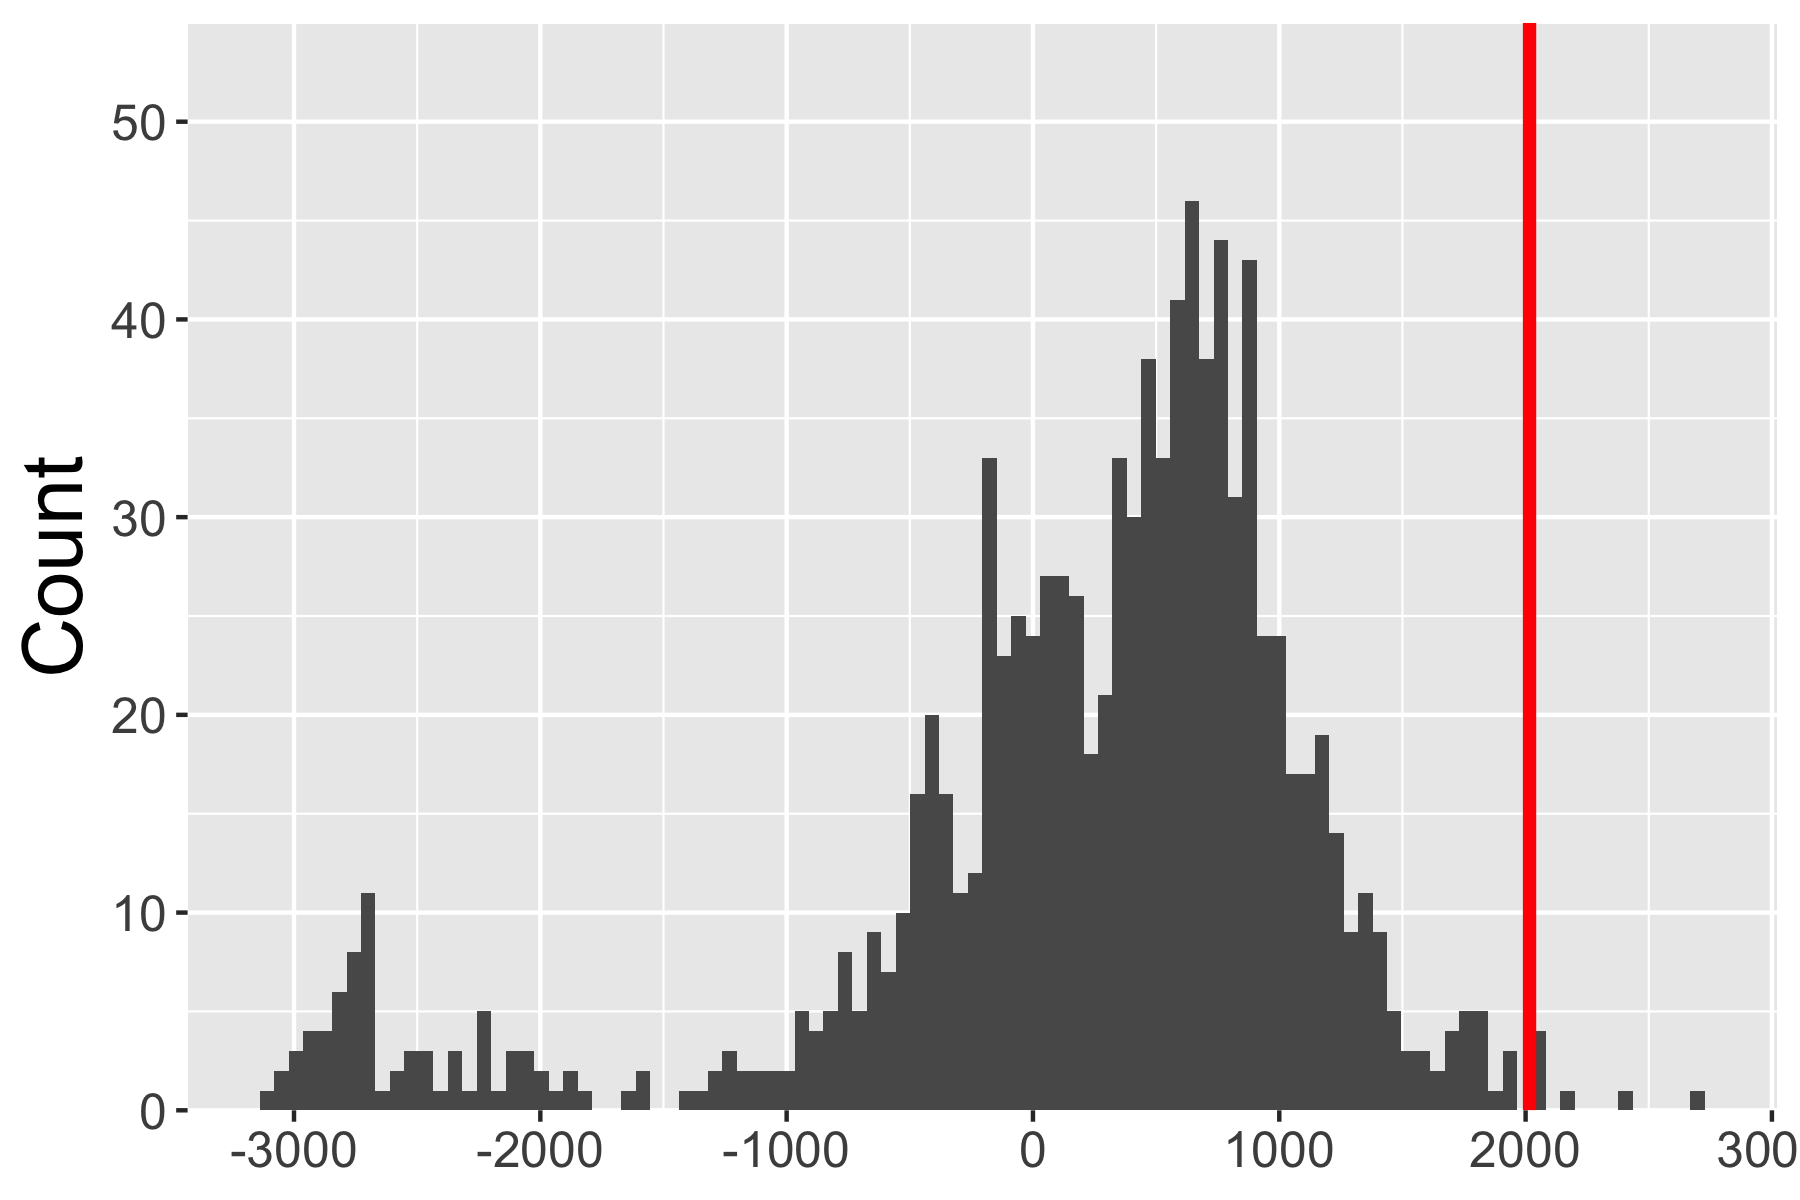
\includegraphics[width=0.3\columnwidth, trim={4cm 1cm 3cm 5cm}, clip]{7_conclude/figs/X3.png}
	
	\caption[Functional network differences in Alzheimer's patients vs. controls]{Functional networks exhibiting significant first- and second-order group differences with the corresponding estimated null distribution and alternative statistic (red) using our pipeline  (brain visualization from right).}
\end{figure}

\subsection{Characterizing the Epilepsy Connectome}
Building on the developments adapting these methods to functional MRI,
we deploy and extend the windowed-approaches
to the study of temporal-lobe epilepsy (TLE),
where disease signals are known to
cause widespread disruptions in connectivity dynamics within the well-studied epileptogenic network, 
but it is not yet clear if and to what extent other networks are perturbed in TLE.

Experimentally, we demonstrate that the approach identifies distinct subsets of temporally evolving connectivity features that stratify TLE patients and healthy controls, which map to altered connectivity at the network-scale. 

\begin{figure}
	\centering
	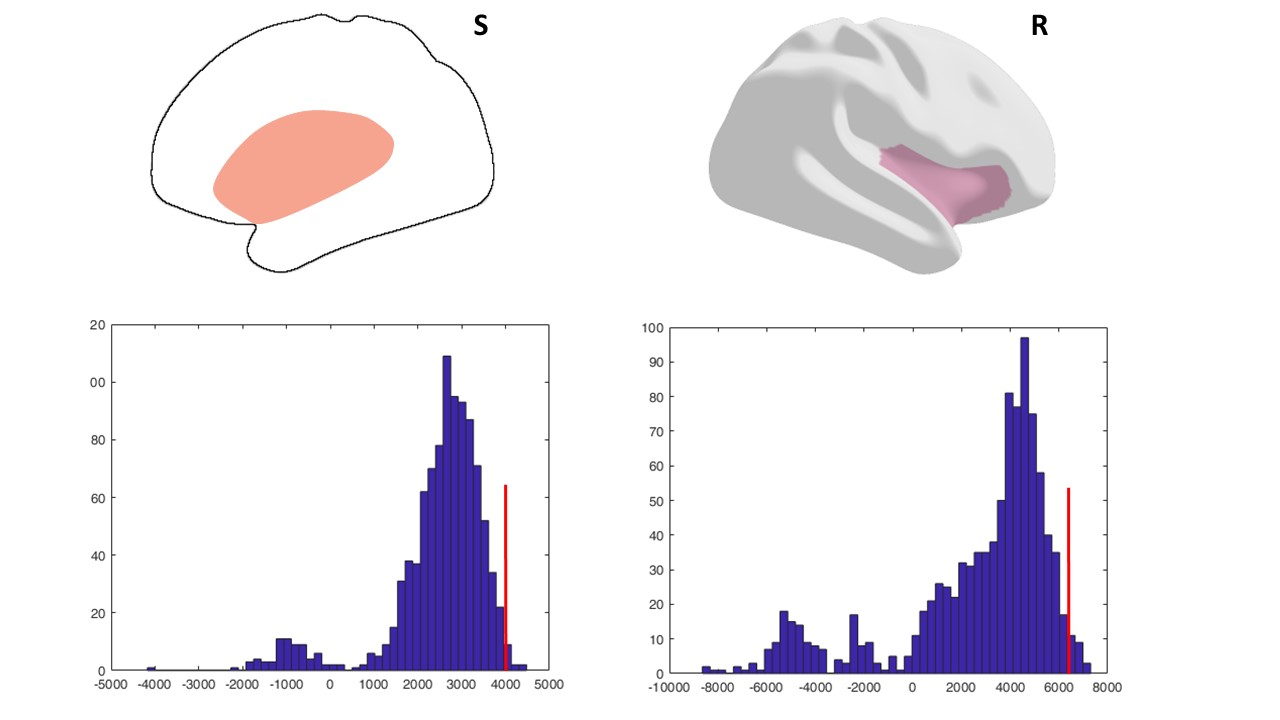
\includegraphics[width=0.45\textwidth, trim={2.5cm 0cm 3cm 0cm}]{7_conclude/figs/ProposedMethod_Results1.jpg}
	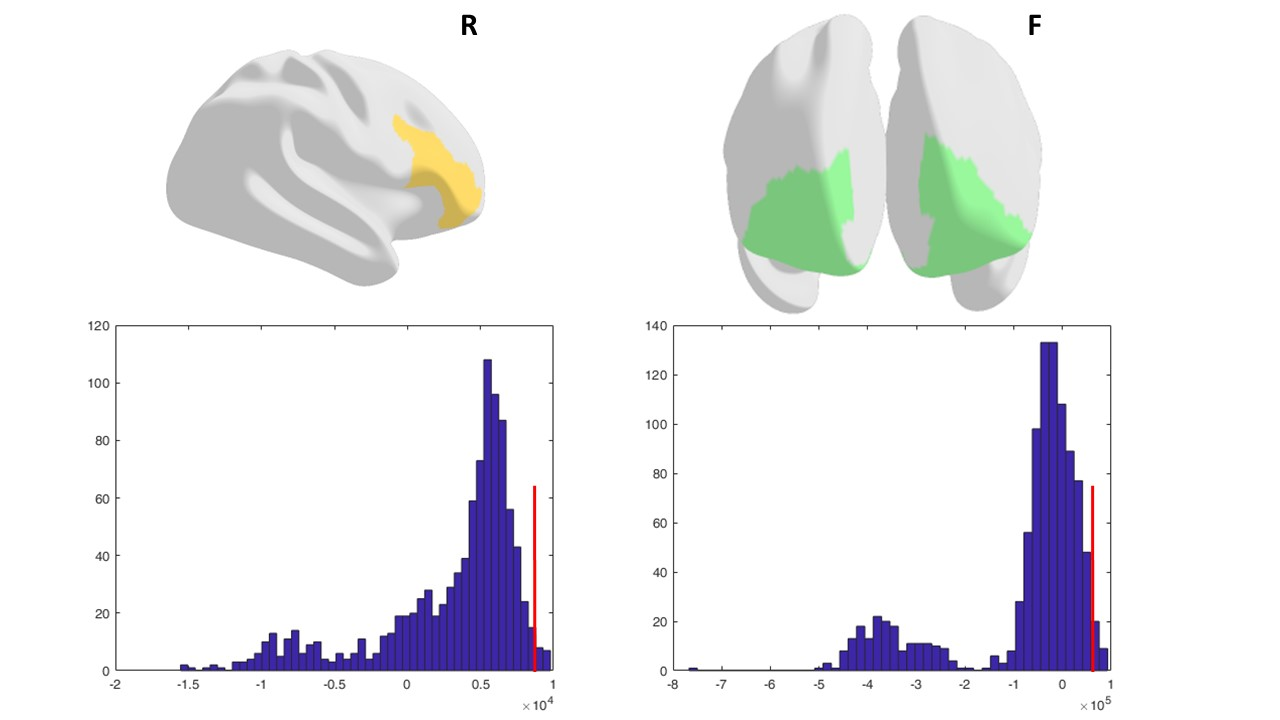
\includegraphics[width=0.45\textwidth, trim={2.5cm 0cm 4cm 0cm},clip]{7_conclude/figs/ProposedMethod_Results2.jpg}
	\caption[Differences in network connectivities in TLE populations]{Networks exhibiting significant first- and second-order group differences using the proposed method with the corresponding estimated null distribution and alternative statistic: (from left to right) Subcortical, Insular and Frontal Opercular Cortex, Inferior Frontal Cortex, Orbital and Polar Frontal Cortex. S - saggital view, R - visualization from the right, F - visualization from the front. \label{fig:CovTrajResults}}
\end{figure}

\section{Building Plug-and-Play Tools for Discrete Optimal Transport}

The rate of development and research in machine learning and associated applications
continues at its current pace
largely due to 
easily deployable tools that
operate seemlessly with existing workflows.
PyTorch, Tensorflow, and all associated software
packages have enabled this growth.
In fact,
concurrent to this work,
a separate group had identified 
similar insights to ours,
and was similarly reviewed and published
with great interest at the same conference~\citep{just2023lava}.
While there have been significant 
developments in Optimal Transport
and its associated 
uses in deep learning,
turnkey tools remain somewhat lacking
for a number of reasons,
as described in Chapter~\ref{chap:demd}.

Building upon the theoretical
efficiencies of the $d$-EMD solver
and minimizer,
we are developing
a plug-in for the Python Optimal Transport library,
with the goal of enabling
optimal transport researchers to 
more easily develop methods
for both pure transportation problems,
as well as methods that incorporate
with automatic differentiation pipelines.
With the ability to solve larger-scale 
problems efficiently,
users can more easily solve 
problems with high-dimensional data
that would otherwise be infeasible
with existing off-the-shelf solvers.

As noted,
the efficient multi-marginal solution
opens the door to a large number 
of domains unstudied due to computational cost.
With approachable open-source code
we hope to expand the tools described
beyond one-dimensional distributions
to problems in computer vision,
both over two dimensional image spaces
as well as beyond.
New computational bottlenecks may arise
as the distributions become
higher-order tensors, which 
may themselves lead to 
the need for new technical
insight.

Building upon the applications in fairness
and the ideas related to subgroup fairness
mentioned at the end of Chapter~\ref{chap:demd},
we hope to specifically
develop and merge existing fairness
software stacks with our tools.
Theoretically, subgroup fairness implies
particular relationships among distributions,
and as such interesting algorithmic
and computational tools may be enabled
under assumptions typical in subgroup settings.


\section{Interpretability in Deep Models}\label{sec:latents}
\todo{ongoing/future work on latent spaces and condindep}
Work in unlearning in Chapter~\ref{chap:lcodec} is relatively nascent,
but excitement in the field is growing
and a number of works have been motivated
by recent successes.
Methods for directly measuring, and perhaps
even promoting or reducing conditional
independence are beginning to be explored.
Motivated by the discretization ideas
in Chapter~\ref{chap:demd} alongside
conditional independence,
a particular direction of interest
is that of general interpretability 
within continuous and typically
black-box models.
When a system is a large,
complex function with high dimension
and nonlinearity,
expecting sparse solutions
that \textit{also} correspond
to clear demarcations within the task or 
data is extremely optimistic.
Using methods described in the introduction
such as activation maps
or Shapley values typically 
leads to some form of ``blame"
in a continuous sense;
this feature or parameter
has the \textit{largest} influence,
but it is not, or we cannot say,
that it is the \textit{only} influence.
Conditional independence is exactly
the measure we are interested in,
and equipped with a reasonable measure,
it seems promising to explore its
application within the broader space of
interpretability.

\subsection{A Final Note}
As noted, current state-of-the-art
machine learning research
is moving at an accelerating pace.
During the time of putting
together this text,
previously promising directions
of research interest in the community
have come and gone.
The exceptional performance
of transformer models
has spurred exponential developments
in language models,
bleeding into vision domains
where previous work primarily
focused on convolutional methods.

The field is now at a point
where almost all high-visibility
work can only be done
with large language models.
The development and deployment
of GPT-2, ChatGPT, and its contemporaries
has all but enveloped interest
in artificial intelligence and machine learning.
While the ideas above could be independently
researched,
it is almost a requirement that now they 
all be developed with application to large
language models in mind.

Importantly, this accelerating pace
of innovation does not appear to be slowing,
and it is difficult to predict
what will be the most important
new development, given timelines
for real-world performance beating
state=of-the-art is now on the order of months.

THe excitement of these developments notwithstanding,
concerns surrounding ideas motivating this thesis
are becoming more and more important as well
as evident, with respect to fairness,
accountability, and safety.
Aligning models to the goals of stakeholders
is of increasing importance as the models'
ability to affect the world grows,
and I hope that we as machine learning
researchers, and as humans, rise to the task.